\documentclass{article}
\usepackage[english]{babel}
\usepackage{amsmath,amssymb,graphicx,enumerate,bbm,hyperref,latexsym,theorem}

%%%%%%%%%% Start TeXmacs macros
\catcode`\<=\active \def<{
\fontencoding{T1}\selectfont\symbol{60}\fontencoding{\encodingdefault}}
\catcode`\>=\active \def>{
\fontencoding{T1}\selectfont\symbol{62}\fontencoding{\encodingdefault}}
\newcommand{\assign}{:=}
\newcommand{\nin}{\not\in}
\newcommand{\nobracket}{}
\newcommand{\tmdummy}{$\mbox{}$}
\newcommand{\tmop}[1]{\ensuremath{\operatorname{#1}}}
\newcommand{\tmtextit}[1]{{\itshape{#1}}}
\newenvironment{enumeratenumeric}{\begin{enumerate}[1.] }{\end{enumerate}}
\newenvironment{proof}{\noindent\textbf{Proof\ }}{\hspace*{\fill}$\Box$\medskip}
{\theorembodyfont{\rmfamily}\newtheorem{answer}{Answer}}
\newtheorem{corollary}{Corollary}
\newtheorem{definition}{Definition}
{\theorembodyfont{\rmfamily}\newtheorem{question}{Question}}
{\theorembodyfont{\rmfamily}\newtheorem{remark}{Remark}}
\newtheorem{theorem}{Theorem}
%%%%%%%%%% End TeXmacs macros

%

%


\begin{document}

'March 4, 2017

\begin{question}
  \label{q1}How does the statement of Proposition 6.4
  \[ \begin{array}{l}
       \int_{- 1}^1 \int_{- 1}^1 \int_{- 1}^1 (1 - u^2)^{\frac{q - 2}{2}} (1 -
       v^2)^{\frac{\lambda + \nu - q}{2} - 1} (1 - w^2)^{\frac{p - 3}{2}} | w
       |^{\lambda + \nu - n} | u - v |^{- \nu} \times\\
       \qquad \times \tilde{C}^{\frac{p}{2} - 1}_{a'} \left( \frac{v}{\sqrt{1
       - w^2 (1 - v^2)}} \right) (1 - w^2 (1 - v^2))^{\frac{a'}{2}}
       \widetilde{\tilde{C}}^{\frac{q - 1}{2}}_b (u)
       \widetilde{\tilde{C}}^{\frac{p - 1}{2} + a'}_{a - a'} \left( \sqrt{w^2
       (1 - v^2)} \right) d u d v d w,
     \end{array} \]
  changes, if in the integral we do variable change $(u, v, w) \rightarrow (u,
  v, z)$ with $z = \sqrt{1 - w^2 (1 - v^2)}$?
\end{question}

\begin{answer}
  It becomes: 
\end{answer}
\begin{eqnarray}
  & \int_D (1 - u^2)^{\frac{q - 2}{2}} (z^2 - v^2)^{\frac{p - 3}{2}} (1 -
  z^2)^{\frac{\lambda + \nu - n - 1}{2}} | u - v |^{- \nu}
  \tilde{C}^{\frac{p}{2} - 1}_{a'} \left( \frac{v}{z} \right) z^{a' + 1}
  \widetilde{\tilde{C}}^{\frac{q - 1}{2}}_b (u) \widetilde{\tilde{C}}^{\frac{p
  - 1}{2} + a'}_{a - a'} \left( \sqrt{1 - z^2} \right) = &  \nonumber\\
  & = \frac{\Gamma \left( \frac{a' + b + \nu}{2} \right) \Gamma \left(
  \frac{1 - \nu}{2} \right) \Gamma \left( \frac{\lambda - \nu}{2} \right)
  \Gamma \left( \frac{1 + \lambda + \nu - n}{2} \right)}{\Gamma \left(
  \frac{\nu}{2} \right) \Gamma \left( \frac{1 - a' + b - \nu + q}{2} \right)
  \Gamma \left( \frac{a' + b + \lambda}{2} \right)  \hspace{0.17em} \Gamma
  \left( \frac{1 + a' - b + \lambda - q}{2} \right)} \times \tilde{c}_{p, q,
  a', a, b} &  \nonumber\\
  & \;_4 F_3 \left( \begin{array}{c}
    \frac{\lambda - \nu}{2}, \frac{a' - a}{2}, \frac{\lambda + \nu - n +
    1}{2}, \frac{p - 1 + a' + a}{2}\\
    \frac{a' + b + \lambda}{2}, \frac{1}{2}, \frac{1 + a' - b + \lambda -
    q}{2}
  \end{array} ; 1 \right) &  \nonumber
\end{eqnarray}
where
\begin{eqnarray}
  & D \assign \{ (u, v, z) \in [- 1, 1] \times [0, 1]^2 \mid v \leqslant z
  \}, &  \nonumber\\
  & \tilde{c}_{p, q, a', a, b} : = c_{p, q, a', a, b} / 2. &  \nonumber
\end{eqnarray}
and $c_{p, q, a', a, b} \neq 0$ is the constant depending only on $(p, q, a',
a, b)$, the one mentioned in Proposition 6.4.

\begin{question}
  How does the equality of Question 1 changes if we use unnormalized
  Gegenbauer polynomials?
\end{question}

Recall that
\begin{eqnarray}
  & \widetilde{\tilde{C}}^{\mu}_N (t) = \left( \mu + \frac{N}{2} \right)
  \Gamma (\mu) C^{\mu}_N (t) &  \nonumber\\
  & \tilde{C}_N^{\mu} (t) = \frac{\Gamma (\mu)}{\Gamma \left( \mu + \left[
  \frac{N}{2} \right] \right)} C^{\mu}_N (t) . &  \nonumber
\end{eqnarray}
Hence
\[ \begin{array}{l}
     \int_{- 1}^1 \int_{- 1}^1 \int_{- 1}^1 (1 - u^2)^{\frac{q - 2}{2}} (1 -
     v^2)^{\frac{\lambda + \nu - q}{2} - 1} (1 - w^2)^{\frac{p - 3}{2}} | w
     |^{\lambda + \nu - n} | u - v |^{- \nu} \times\\
     \qquad \times \tilde{C}^{\frac{p}{2} - 1}_{a'} \left( \frac{v}{\sqrt{1 -
     w^2 (1 - v^2)}} \right) (1 - w^2 (1 - v^2))^{\frac{a'}{2}}
     \widetilde{\tilde{C}}^{\frac{q - 1}{2}}_b (u)
     \widetilde{\tilde{C}}^{\frac{p - 1}{2} + a'}_{a - a'} \left( \sqrt{w^2 (1
     - v^2)} \right) d u d v d w =\\
     = \frac{\Gamma \left( \frac{p - 2}{2} \right) \Gamma \left( \frac{q -
     1}{2} \right) \left( \frac{q - 1 + b}{2} \right) \Gamma \left( \frac{p -
     1}{2} + a' \right) \left( \frac{p - 1}{2} + \frac{a + a'}{2}
     \right)}{\Gamma \left( \frac{p - 2}{2} + \left[ \frac{a'}{2} \right]
     \right)} \times\\
     \times \int_{- 1}^1 \int_{- 1}^1 \int_{- 1}^1 (1 - u^2)^{\frac{q - 2}{2}}
     (1 - v^2)^{\frac{\lambda + \nu - q}{2} - 1} (1 - w^2)^{\frac{p - 3}{2}} |
     w |^{\lambda + \nu - n} | u - v |^{- \nu} \times\\
     \qquad \times C^{\frac{p}{2} - 1}_{a'} \left( \frac{v}{\sqrt{1 - w^2 (1 -
     v^2)}} \right) (1 - w^2 (1 - v^2))^{\frac{a'}{2}}
     \widetilde{\tilde{C}}^{\frac{q - 1}{2}}_b (u)
     \widetilde{\tilde{C}}^{\frac{p - 1}{2} + a'}_{a - a'} \left( \sqrt{w^2 (1
     - v^2)} \right) d u d v d w.
   \end{array} \]
Therefore, the equality in Question 1 becomes
\begin{eqnarray}
  & \int_D (1 - u^2)^{\frac{q - 2}{2}} (z^2 - v^2)^{\frac{p - 3}{2}} (1 -
  z^2)^{\frac{\lambda + \nu - n - 1}{2}} | u - v |^{- \nu} C^{\frac{p}{2} -
  1}_{a'} \left( \frac{v}{z} \right) z^{a' + 1} C^{\frac{q - 1}{2}}_b (u)
  C^{\frac{p - 1}{2} + a'}_{a - a'} \left( \sqrt{1 - z^2} \right) = & 
  \nonumber\\
  & = \frac{\Gamma \left( \frac{a' + b + \nu}{2} \right) \Gamma \left(
  \frac{1 - \nu}{2} \right) \Gamma \left( \frac{\lambda - \nu}{2} \right)
  \Gamma \left( \frac{1 + \lambda + \nu - n}{2} \right)}{\Gamma \left(
  \frac{\nu}{2} \right) \Gamma \left( \frac{1 - a' + b - \nu + q}{2} \right)
  \Gamma \left( \frac{a' + b + \lambda}{2} \right)  \hspace{0.17em} \Gamma
  \left( \frac{1 + a' - b + \lambda - q}{2} \right)} \times \frac{\Gamma
  \left( \frac{p - 2}{2} \right) \Gamma \left( \frac{q - 1}{2} \right) \left(
  \frac{q - 1 + b}{2} \right) \Gamma \left( \frac{p - 1}{2} + a' \right)
  \left( \frac{p - 1}{2} + \frac{a + a'}{2} \right)}{\Gamma \left( \frac{p -
  2}{2} + \left[ \frac{a'}{2} \right] \right)} \times \tilde{c}_{p, q, a', a,
  b} &  \nonumber\\
  & \;_4 F_3 \left( \begin{array}{c}
    \frac{\lambda - \nu}{2}, \frac{a' - a}{2}, \frac{\lambda + \nu - n +
    1}{2}, \frac{p - 1 + a' + a}{2}\\
    \frac{a' + b + \lambda}{2}, \frac{1}{2}, \frac{1 + a' - b + \lambda -
    q}{2}
  \end{array} ; 1 \right) &  \nonumber
\end{eqnarray}
\begin{question}
  In the statement of Proposition 6.4, is it essential that $(p, q) \in
  \mathbbm{N}_+$?
\end{question}

\begin{answer}
  No, we can assume barely $p, q \in \mathbbm{C}$ (note that the
  domain-of-convergence part of Proposition 6.4 will change accordingly).
\end{answer}

\begin{question}
  What does the integral in Question \ref{q1} becomes if we do variable
  substitution
  \[ \left\{ \begin{array}{l}
       u = \theta,\\
       \frac{v}{z} = \cos \psi,\\
       z = \cos \varphi ?
     \end{array} \right. \]
\end{question}

\begin{answer}
  As we have
  \[ \frac{\partial (u, v, z)}{\partial (\theta, \psi, \varphi)} =
     \left|\begin{array}{ccc}
       \cos \theta & 0 & 0\\
       0 & - \cos \varphi \sin \psi & - \sin \varphi \cos \psi\\
       0 & 0 & - \sin \varphi
     \end{array}\right| = \cos (\theta) \sin (\varphi) \cos (\varphi) \sin
     (\psi), \]
  it becomes:
  \begin{eqnarray}
    & \int_{- \pi / 2}^{\pi / 2} \int_0^{\pi / 2} \int_0^{\pi / 2} \cos^{q -
    1} (\theta) \cos^{p - 1 + a'} (\varphi) \sin^{p - 2} (\psi) \sin^{\lambda
    + \nu - n} \varphi | \sin \theta - \cos \psi \cos \varphi |^{- \nu} & 
    \nonumber\\
    & \widetilde{\tilde{C}}^{\frac{q - 1}{2}}_b (\sin \theta)
    \tilde{C}^{\frac{p}{2} - 1}_{a'} (\cos \psi)
    \widetilde{\tilde{C}}^{\frac{p - 1}{2} + a'}_{a - a'} (\sin \varphi) d
    \psi d \varphi d \theta . &  \nonumber
  \end{eqnarray}
\end{answer}

\begin{definition}
  We let $\tilde{\Gamma} (x) \assign \Gamma (x)$ if $x \nin -\mathbbm{N}$ and
  $\assign 1$ otherwise.
\end{definition}

\begin{question}
  What becomes to previous question when we introduce the following notation:
  \begin{eqnarray}
    & v_l^{\lambda} (\theta) \assign (\sin \theta)^{2 \lambda} C^{\lambda}_l
    (\cos \theta) &  \nonumber\\
    & \frac{q - 1}{2} \rightsquigarrow \lambda, & b \rightsquigarrow l,
    \nonumber\\
    & \frac{p}{2} - 1 \rightsquigarrow \mu, & a' \rightsquigarrow m,
    \nonumber\\
    & \frac{p - 1}{2} + a' \rightsquigarrow \nu, & a - a' \rightsquigarrow n,
    \nonumber\\
    & \lambda + \nu - (p + q) \rightsquigarrow a, & \nu \rightsquigarrow b ?
    \nonumber
  \end{eqnarray}
\end{question}

\begin{answer}
  We have
  \begin{eqnarray}
    & n \rightsquigarrow 2 \lambda + 2 \mu + 3 &  \nonumber\\
    & \lambda - \nu \rightsquigarrow a + 2 \lambda + 2 \mu + 3 - 2 b & 
    \nonumber\\
    & \lambda \rightsquigarrow a + 2 \lambda + 2 \mu + 3 - b &  \nonumber
  \end{eqnarray}
  Hence, it becomes
  \begin{eqnarray}
    & \Gamma (\lambda) \Gamma (\nu) \Gamma (\nu + n / 2) (- 1)^b \times & 
    \nonumber\\
    & \int_0^{\pi} \int_0^{\pi / 2} \int_0^{\pi / 2} \sin^{- m} (\varphi)
    \cos^a \varphi | \cos \theta - \cos \psi \sin \varphi |^{- b}
    v^{\lambda}_l (\theta) v_m^{\mu} (\psi) v_n^{\nu} (\varphi) d \psi d
    \varphi d \theta = &  \nonumber\\
    & = \frac{\Gamma \left( \frac{m + l + b}{2} \right) \Gamma \left( \frac{1
    - b}{2} \right) \Gamma \left( \frac{a + 2 \lambda + 2 \mu + 3 - 2 b}{2}
    \right) \Gamma \left( \frac{1 + a}{2} \right)}{\Gamma \left( \frac{b}{2}
    \right) \Gamma \left( \frac{2 - m + l - b + 2 \lambda}{2} \right) \Gamma
    \left( \frac{m + l + a + 2 \lambda + 2 \mu + 3 - b}{2} \right) 
    \hspace{0.17em} \Gamma \left( \frac{m - l + a + 2 \mu + 3 - b}{2} \right)}
    &  \nonumber\\
    & \frac{(2 \mu)_{m + n} (- 1)^{\frac{m - l}{2}}}{\Gamma (1 + n / 2)
    \Gamma (m + 1) \Gamma (l + 1)} \left. \times \pi \Gamma \left( \mu +
    \frac{3}{2} + \frac{n}{2} \right) \tilde{\Gamma} \left( \mu + \frac{1}{2}
    \right) \Gamma (2 \lambda + l) 2^{- 2 \lambda} \right. \times & 
    \nonumber\\
    &  &  \nonumber\\
    & \;_4 F_3 \left( \begin{array}{c}
      \frac{a + 2 \lambda + 2 \mu + 3 - 2 b}{2}, - \frac{n}{2}, \frac{a +
      1}{2}, \mu + n / 2\\
      \frac{m + l + a + 2 \lambda + 2 \mu + 3 - b}{2}, \frac{1}{2}, \frac{m -
      l + a + 2 \mu + 3 - b}{2}
    \end{array} ; 1 \right) . &  \nonumber
  \end{eqnarray}
\end{answer}

The conditions are:
\begin{eqnarray}
  & \lambda, \mu, \nu \in \mathbbm{C}; \quad a, b \in \mathbbm{C}; \quad l, m
  \in \mathbbm{N}, n \in 2\mathbbm{N}; &  \nonumber\\
  & l + m \in 2\mathbbm{N}, \quad \nu - \mu = m + \frac{1}{2} . &  \nonumber
\end{eqnarray}
\begin{remark}
  Note that all the manipulatons done in Question 5 and prior to it make sense
  only under the assumption $p > 1$ (nevertheless, for $p = 1$ similar
  manipulations can be introduced).
\end{remark}

\begin{question}
  Are any particular cases of the
  \begin{eqnarray}
    & \int_D (1 - u^2)^{\alpha} (1 - v^2)^{\mu + \beta} (1 - w)^{\beta -
    \frac{1}{2}} | w |^{\mu - \frac{1}{2}} | u - v |^{- \nu}
    \tilde{C}^{\beta}_{a'} (v, 1 - w (1 - v^2)) \widetilde{\tilde{C}}^{\alpha
    - \frac{1}{2}}_b (u) d u d v d w, &  \nonumber\\
    & D \assign \{ (u, v, w) \in [- 1, 1]^2 \times [0, 1] \} . &  \nonumber\\
    & \alpha, \beta, \mu, \nu \in \mathbbm{C}; \quad a', b \in \mathbbm{N}
    \mid a + b \in 2\mathbbm{N}. &  \nonumber
  \end{eqnarray}
  Now, the known special cases of the latter integral are a
  
  quation in question 6 are known?
\end{question}

To my current knowledge, the known cases are:
\begin{enumerate}
  \item The partial case $l = m = n = 0$ is Proposition 6.1;
\end{enumerate}
\begin{definition}
  For $x, y \in \mathbbm{C}$ we let
  \begin{eqnarray}
    & B (x, y) \assign \frac{\Gamma (x) \Gamma (y)}{\Gamma (x + y)} \int_0^1
    (1 - t)^{x - 1} t^{y - 1} d t. &  \nonumber
  \end{eqnarray}
\end{definition}

\begin{question}
  How does the first equality in Question 8 changes if we do variable change:
  \begin{eqnarray}
    & \left[ \begin{array}{c}
      u\\
      v\\
      z
    \end{array} \right] \rightsquigarrow \left[ \begin{array}{c}
      \theta = \arccos (u)\\
      \psi = \arccos \left( \frac{v}{\sqrt{1 - w (1 - v^2)}} \right)\\
      \varphi = \arcsin \left( \sqrt{1 - w (1 - v^2)} \right)
    \end{array} \right] ? &  \nonumber
  \end{eqnarray}
\end{question}

\begin{answer}
  The inverse transform and Jacobial are
  \begin{eqnarray}
    & u = \cos (\theta), \quad v = \sin (\varphi) \cos (\psi), \quad w =
    \frac{\cos^2 (\varphi)}{1 - \cos^2 \psi \sin^2 \varphi} &  \nonumber\\
    & \frac{\partial (u, v, \omega)}{\partial (\theta, \psi, \varphi)} =
    \frac{2 \cos (\varphi) \sin (\theta) \sin^2 (\varphi) \sin (\psi)}{1 -
    \cos^2 (\psi) \sin^2 (\varphi)} &  \nonumber
  \end{eqnarray}
  Hence the equality becomes is:
  \begin{eqnarray}
    & \int_D \sin^{2 \beta + a' + 1} (\varphi) \cos^{2 \mu} (\varphi) | \cos
    (\theta) - \cos (\psi) \sin (\varphi) |^{- \nu} \tilde{v}^{\beta}_{a'}
    (\psi) \tilde{v}^{\alpha + \frac{1}{2}}_b (\theta) = &  \nonumber\\
    & = \frac{\Gamma \left( \alpha + \frac{1}{2} + \left[ \frac{b + 1}{2}
    \right] \right) \Gamma (\beta)}{\Gamma \left( \beta + \left[ \frac{a' +
    1}{2} \right] \right)} \frac{(2 \beta)_{a'} (- 1)^{\frac{a' - b}{2}} (2
    \alpha + 1)_b}{a' ! b!} \left. \times \pi \Gamma \left( \beta +
    \frac{1}{2} \right) \Gamma (2 \alpha + 1) 2^{- 1 - 2 \alpha} \right.
    \times &  \nonumber\\
    & \frac{\Gamma \left( \frac{a' + b + \nu}{2} \right) \Gamma (\mu - \nu +
    \alpha + \beta + 2) \Gamma (\mu + 1 / 2) \Gamma \left( \frac{1 - \nu}{2}
    \right)}{\Gamma \left( \frac{\nu}{2} \right) \Gamma \left( \frac{3 - a' +
    b - \nu + 2 \alpha}{2} \right)  \hspace{0.17em} \Gamma \left( \frac{a' + b
    + 2 \mu - \nu + 2 \alpha + 2 \beta + 4}{2} \right) \Gamma \left( \frac{a'
    - b + 2 \mu - \nu + 2 \beta + 3}{2} \right)}, &  \nonumber
  \end{eqnarray}
  where $\tilde{v}_l^{\lambda} (\theta) \assign (\sin \theta)^{2 \lambda}
  \tilde{C}^{\lambda}_l (\cos \theta)$ and $D \assign \left\{ (\theta, \psi,
  \varphi) \in [0, \pi] \times \left[ 0, \frac{\pi}{2} \right]^2 \right\}$.
  
  If we further do the substitutions
  \begin{eqnarray}
    & a' \rightsquigarrow a, \quad \alpha + \frac{1}{2} \rightsquigarrow
    \beta, \quad \beta \rightsquigarrow \alpha, &  \nonumber
  \end{eqnarray}
  it becomes
  \begin{eqnarray}
    & \int_D \sin^{2 \alpha + a + 1} (\varphi) \cos^{2 \mu} (\varphi) | \cos
    (\theta) - \cos (\psi) \sin (\varphi) |^{- \nu} \tilde{v}^{\alpha}_a
    (\psi) \tilde{v}^{\beta}_b (\theta) = \hspace*{\fill} &  \nonumber\\
    & = \frac{2^{a + b - 1} \Gamma \left( \alpha + \frac{1}{2} + \left[
    \frac{a}{2} \right] \right) (- 1)^{\frac{a - b}{2}} \sqrt{\pi} \Gamma
    \left( \beta + [b / 2] + \frac{1}{2} \right)}{a! b!} \nobracket \nobracket
    &  \nonumber\\
    & \frac{\Gamma \left( \frac{a + b + \nu}{2} \right) \Gamma (\mu - \nu +
    \alpha + \beta + 3 / 2) \Gamma (\mu + 1 / 2) \Gamma \left( \frac{1 -
    \nu}{2} \right)}{\Gamma \left( \frac{\nu}{2} \right) \Gamma \left( \frac{a
    + b + 2 \mu - \nu + 2 \alpha + 2 \beta + 3}{2} \right) \Gamma \left(
    \frac{2 - a + b - \nu + 2 \beta}{2} \right) \Gamma \left( \frac{a - b + 2
    \mu - \nu + 2 \alpha + 3}{2} \right)}, &  \nonumber
  \end{eqnarray}
  or using the beta function defined above,
  \begin{eqnarray}
    & \int_D \sin^{2 \alpha + a + 1} (\varphi) \cos^{2 \mu} (\varphi) | \cos
    (\theta) - \cos (\psi) \sin (\varphi) |^{- \nu} \tilde{v}^{\alpha}_a
    (\psi) \tilde{v}^{\beta}_b (\theta) = \hspace*{\fill} &  \nonumber\\
    & = \frac{2^{a + b - 1} \Gamma \left( \alpha + \frac{1}{2} + \left[
    \frac{a}{2} \right] \right) (- 1)^{\frac{a - b}{2}} \sqrt{\pi} \Gamma
    \left( \beta + \left[ \frac{b}{2} \right] + \frac{1}{2} \right)}{a! b!}
    \nobracket \nobracket &  \nonumber\\
    & \frac{B \left( \frac{a + b + \nu}{2}, \mu - \nu + \alpha + \beta + 3 /
    2 \right) \Gamma (\mu + 1 / 2) \Gamma \left( \frac{1 - \nu}{2}
    \right)}{\Gamma \left( \frac{\nu}{2} \right) \Gamma \left( \frac{2 - a + b
    - \nu + 2 \beta}{2} \right) \Gamma \left( \frac{a - b + 2 \mu - \nu + 2
    \alpha + 3}{2} \right)} . &  \nonumber
  \end{eqnarray}
  Finally, making the substitution:
  \begin{eqnarray}
    & \beta \rightsquigarrow \lambda, b \rightsquigarrow l, \alpha
    \rightsquigarrow \mu, a \rightsquigarrow m, \mu \rightsquigarrow a / 2,
    \nu \rightsquigarrow b, &  \nonumber
  \end{eqnarray}
  we get
  \begin{eqnarray}
    & \int_D \sin^{2 \mu + m + 1} (\varphi) \cos^a (\varphi) | \cos (\theta)
    - \cos (\psi) \sin (\varphi) |^{- b} \tilde{v}^{\lambda}_l (\theta)
    \tilde{v}^{\mu}_m (\psi) d \theta d \psi d \varphi = \hspace*{\fill} & 
    \nonumber\\
    & = \frac{2^{m + l - 1} (- 1)^{\frac{m - l}{2}} \sqrt{\pi} \Gamma \left(
    \mu + \frac{1}{2} + \left[ \frac{m}{2} \right] \right) \Gamma \left(
    \lambda + \left[ \frac{l}{2} \right] + \frac{1}{2} \right)}{a! b!}
    \nobracket \nobracket \times  \label{eq-2} & \\
    & \frac{\Gamma \left( \frac{m + l + b}{2} \right) \Gamma \left( \frac{a -
    2 b + 2 \mu + 2 \lambda + 3}{2} \right) \Gamma \left( \frac{a + 1}{2}
    \right) \Gamma \left( \frac{1 - b}{2} \right)}{\Gamma \left( \frac{b}{2}
    \right) \Gamma \left( \frac{m + l + a - b + 2 \mu + 2 \lambda + 3}{2}
    \right) \Gamma \left( \frac{2 - m + l - b + 2 \lambda}{2} \right) \Gamma
    \left( \frac{m - l + a - b + 2 \mu + 3}{2} \right)} . &  \nonumber
  \end{eqnarray}
  or
  \begin{eqnarray}
    & \int_D \sin^{2 \mu + m + 1} (\varphi) \cos^a (\varphi) | \cos (\theta)
    - \cos (\psi) \sin (\varphi) |^{- b} \tilde{v}^{\lambda}_l (\theta)
    \tilde{v}^{\mu}_m (\psi) d \theta d \psi d \varphi = \hspace*{\fill} & 
    \nonumber\\
    & = \frac{2^{m + l - 1} (- 1)^{\frac{m - l}{2}} \sqrt{\pi} \Gamma \left(
    \mu + \frac{1}{2} + \left[ \frac{m}{2} \right] \right) \Gamma \left(
    \lambda + \left[ \frac{l}{2} \right] + \frac{1}{2} \right)}{a! b!}
    \nobracket \nobracket \times &  \nonumber\\
    & \frac{B \left( \frac{m + l + b}{2}, \frac{a - 2 b + 2 \mu + 2 \lambda +
    3}{2} \right) \Gamma \left( \frac{a + 1}{2} \right) \Gamma \left( \frac{1
    - b}{2} \right)}{\Gamma \left( \frac{b}{2} \right) \Gamma \left( \frac{2 -
    m + l - b + 2 \lambda}{2} \right) \Gamma \left( \frac{m - l + a - b + 2
    \mu + 3}{2} \right)} . &  \nonumber\\
    & \lambda, \mu, a, b \in \mathbbm{C}; \quad l, m \in \mathbbm{N} \mid l +
    m \in 2\mathbbm{N} &  \nonumber
  \end{eqnarray}
\end{answer}

\begin{question}
  Which specializations of integral in Question 7 are previously known?
\end{question}

\begin{definition}
  For $\mu \in \mathbbm{C}, N \in \mathbbm{N}$, let polynomial
  $\tilde{C}_N^{\mu} (s, t)$ be defined as
  \begin{eqnarray}
    & \tilde{C}_N^{\mu} (s, t) \assign \frac{\Gamma (\mu)}{\Gamma \left( \mu
    + \left[ \frac{N + 1}{2} \right] \right)} C \left( \frac{s}{\sqrt{t}}
    \right) t^{N / 2} . &  \nonumber
  \end{eqnarray}
\end{definition}

\begin{answer}
  For simplicity, we shall use the $(u, v, w)$-variables from Question 1:
  \begin{eqnarray}
    & \int_{- 1}^1 \int_{- 1}^1 \int_{- 1}^1 (1 - u^2)^{\frac{q - 2}{2}} (1 -
    v^2)^{\frac{\lambda + \nu - q}{2} + N - 1} (1 - w^2)^{\frac{p - 3}{2}} | w
    |^{\lambda + \nu - n + 2 N} | u - v |^{- \nu} \tilde{C}^{\frac{p}{2} -
    1}_{a'} \left( v, \sqrt{1 - w^2 (1 - v^2)} \right)
    \widetilde{\tilde{C}}^{\frac{q - 1}{2}}_b (u) d u d v d w. &  \nonumber
  \end{eqnarray}
  We also do the parameter and variable substitutions,
  \begin{eqnarray}
    & w^2 \rightsquigarrow w, \frac{\lambda + \nu - n}{2} + N
    \rightsquigarrow \mu, \frac{p - 2}{2} \rightsquigarrow \beta, \frac{q -
    2}{2} \rightsquigarrow \alpha &  \nonumber
  \end{eqnarray}
  so to get
  \begin{eqnarray}
    & \int_D (1 - u^2)^{\alpha} (1 - v^2)^{\mu + \beta} (1 - w)^{\beta -
    \frac{1}{2}} | w |^{\mu - \frac{1}{2}} | u - v |^{- \nu}
    \tilde{C}^{\beta}_{a'} (v, 1 - w (1 - v^2)) \tilde{C}^{\alpha +
    \frac{1}{2}}_b (u, 1) d u v w = &  \nonumber\\
    & \frac{2^{a' + b} \Gamma \left( \beta + \frac{1}{2} + \left[ \frac{a' +
    1}{2} \right] \right) \Gamma \left( \alpha + 1 + \left[ \frac{b + 1}{2}
    \right] \right) (- 1)^{\frac{a' - b}{2}} \sqrt{\pi}}{a' ! b!} \cdot
    \frac{B \left( \frac{a' + b + \nu}{2}, \mu - \nu + \alpha + \beta + 2
    \right) \Gamma \left( \mu + \frac{1}{2} \right) \Gamma \left( \frac{1 -
    \nu}{2} \right)}{\Gamma \left( \frac{\nu}{2} \right) \Gamma \left( \frac{3
    - a' + b - \nu + 2 \alpha}{2} \right) \Gamma \left( \frac{a' - b + 2 \mu -
    \nu + 2 \beta + 3}{2} \right)} \label{eq:q8-1}  & \\
    & D \assign \{ (u, v, w) \in [- 1, 1]^2 \times [0, 1] \} . &  \nonumber\\
    & \alpha, \beta, \mu, \nu \in \mathbbm{C}; \quad a', b \in \mathbbm{N}
    \mid a + b \in 2\mathbbm{N}. &  \nonumber
  \end{eqnarray}
  We further do the substitutions:
  \begin{eqnarray}
    & a' \rightsquigarrow m, \alpha + \frac{1}{2} \rightsquigarrow \lambda,
    \mu \rightsquigarrow a / 2, \beta \rightsquigarrow \mu, b \rightsquigarrow
    l, \nu \rightsquigarrow b &  \nonumber
  \end{eqnarray}
  to get
  \begin{eqnarray}
    & \int_D (1 - u^2)^{\lambda - \frac{1}{2}} (1 - v^2)^{\frac{a}{2} + \mu}
    (1 - w)^{\mu - \frac{1}{2}} | w |^{\frac{a - 1}{2}} | u - v |^{- b}
    \tilde{C}^{\mu}_m (v, 1 - w (1 - v^2)) \tilde{C}^{\lambda}_l (u, 1) d u v
    w = &  \nonumber\\
    & \frac{2^{m + l} \Gamma \left( \mu + \frac{1}{2} + \left[ \frac{m}{2}
    \right] \right) \Gamma \left( \lambda + \frac{1}{2} + \left[ \frac{l}{2}
    \right] \right) (- 1)^{\frac{m - l}{2}} \sqrt{\pi}}{m!l!} \cdot \frac{B
    \left( \frac{m + l + b}{2}, \frac{a}{2} - b + \lambda + \mu + \frac{3}{2}
    \right) \Gamma \left( \frac{a + 1}{2} \right) \Gamma \left( \frac{1 -
    b}{2} \right)}{\Gamma \left( \frac{b}{2} \right) \Gamma \left( \frac{2 - m
    + l - b + 2 \lambda}{2} \right) \Gamma \left( \frac{m - l + a - b + 2 \mu
    + 3}{2} \right)}  & \\
    & D \assign \{ (u, v, w) \in [- 1, 1]^2 \times [0, 1] \} . &  \nonumber\\
    & \lambda, \mu, a, b \in \mathbbm{C}; \quad m, l \in \mathbbm{N} \mid m +
    l \in 2\mathbbm{N}. &  \nonumber
  \end{eqnarray}
  Now, the known special cases of the latter integral are as follows:
  
  (in parameters of Question 8):
  \begin{enumeratenumeric}
    \item $m = l = 0$: product of beta-integral and integral from Proposition
    6.1 (first item):
    \begin{eqnarray}
      & \int_{- 1}^1 \int_{- 1}^1 (1 - u^2)^{\lambda - \frac{1}{2}} (1 -
      v^2)^{\frac{a}{2} + \mu} | u - v |^{- b} d u d v \times \int_0^1 (1 -
      w)^{\mu - \frac{1}{2}} | w |^{\frac{a - 1}{2}} d w = &  \nonumber\\
      & \frac{\sqrt{\pi} \Gamma (\lambda + \frac{1}{2}) \Gamma \left( \frac{1
      - b}{2} \right) \Gamma (\lambda + \mu + \frac{a}{2} - b +
      \frac{3}{2})}{\Gamma \left( \lambda - \frac{b}{2} + 1 \right) \Gamma
      \left( \mu + \frac{a - b}{2} + \frac{3}{2} \right) \Gamma \left( \lambda
      + \mu + \frac{a - b}{2} + \frac{3}{2} \right)} \cdot B \left( \mu +
      \frac{1}{2}, \frac{a + 1}{2} \right) &  \nonumber
    \end{eqnarray}
    \item $m = l = 1$: product of beta-integral (we let $B (x, y) \assign
    \int_0^1 t^{x - 1} (1 - n)^{y - 1} d t$)) and integral from Proposition
    6.1 (second item):
    \begin{eqnarray}
      & 4 \int_{- 1}^1 \int_{- 1}^1 (1 - u^2)^{\lambda - \frac{1}{2}} (1 -
      v^2)^{\frac{a}{2} + \mu} u v | u - v |^{- b} d u d v \int_0^1 (1 -
      w)^{\mu - \frac{1}{2}} | w |^{\frac{a - 1}{2}} d w = &  \nonumber\\
      & \frac{4 (- b)}{2 \lambda + 1} \int_{- 1}^1 \int_{- 1}^1 (1 -
      u^2)^{\lambda + \frac{1}{2}} (1 - v^2)^{\frac{a}{2} + \mu} v | u - v
      |^{- b - 1} \tmop{sgn} (u - v) d u d v \int_0^1 (1 - w)^{\mu -
      \frac{1}{2}} | w |^{\frac{a - 1}{2}} d w = &  \nonumber\\
      & = \frac{4 b}{2 \lambda + 1} \cdot \frac{\Gamma \left( \frac{1 - b}{2}
      \right) \Gamma \left( \mu + \frac{a}{2} + 1 \right) \Gamma \left(
      \lambda + \frac{3}{2} \right) \Gamma \left( \lambda + \mu - b +
      \frac{a}{2} + \frac{3}{2} \right)}{\Gamma \left( \mu - \frac{a - b +
      3}{2} \right) \Gamma \left( \lambda - \frac{b}{2} + 1 \right) \Gamma
      \left( \lambda + \mu + \frac{a - b + 5}{2} \right)} \cdot B \left( \mu +
      \frac{1}{2}, \frac{a + 1}{2} \right) &  \nonumber
    \end{eqnarray}
  \end{enumeratenumeric}
  (in parameters of Question 7):
  \begin{enumeratenumeric}
    \item $m = l = 0$: product of beta-integral and integral from Proposition
    6.1 (first item):
    \begin{eqnarray}
      & \int_D \sin^{2 \mu + m + 1} (\varphi) \cos^a (\varphi) | \cos
      (\theta) - \cos (\psi) \sin (\varphi) |^{- b} \sin^{2 \lambda} (\theta)
      \sin^{2 \mu} (\psi) d \theta d \psi d \varphi = &  \nonumber\\
      & \frac{\sqrt{\pi} \Gamma (\lambda + \frac{1}{2}) \Gamma \left( \frac{1
      - b}{2} \right) \Gamma (\lambda + \mu + \frac{a}{2} - b +
      \frac{3}{2})}{2 \Gamma \left( \lambda - \frac{b}{2} + 1 \right) \Gamma
      \left( \mu + \frac{a - b}{2} + \frac{3}{2} \right) \Gamma \left( \lambda
      + \mu + \frac{a - b}{2} + \frac{3}{2} \right)} \cdot B \left( \mu +
      \frac{1}{2}, \frac{a + 1}{2} \right) &  \nonumber
    \end{eqnarray}
    \item $m = l = 1$: product of beta-integral (we let $B (x, y) \assign
    \int_0^1 t^{x - 1} (1 - n)^{y - 1} d t$)) and integral from Proposition
    6.1 (second item):
    \begin{eqnarray}
      & \int_D \sin^{2 \mu + m + 1} (\varphi) \cos^a (\varphi) | \cos
      (\theta) - \cos (\psi) \sin (\varphi) |^{- b} \cos (\theta) \cos (\psi)
      \sin^{2 \lambda} (\theta) \sin^{2 \mu} (\psi) d \theta d \psi d \varphi
      &  \nonumber\\
      & = \frac{2 b}{2 \lambda + 1} \cdot \frac{\Gamma \left( \frac{1 - b}{2}
      \right) \Gamma \left( \mu + \frac{a}{2} + 1 \right) \Gamma \left(
      \lambda + \frac{3}{2} \right) \Gamma \left( \lambda + \mu - b +
      \frac{a}{2} + \frac{3}{2} \right)}{\Gamma \left( \mu - \frac{a - b +
      3}{2} \right) \Gamma \left( \lambda - \frac{b}{2} + 1 \right) \Gamma
      \left( \lambda + \mu + \frac{a - b + 5}{2} \right)} \cdot B \left( \mu +
      \frac{1}{2}, \frac{a + 1}{2} \right) &  \nonumber
    \end{eqnarray}
    \item $b = 0$: going to coordinates of the Question 7, it becomes the
    product of three beta integrals
    \begin{eqnarray}
      & \int_D \sin^{2 \mu + m + 1} (\varphi) \cos^a (\varphi)
      \tilde{v}^{\mu}_m (\psi) \tilde{v}^{\lambda}_l (\theta) = &  \nonumber\\
      & = \frac{\pi \Gamma \left( \mu + \frac{1}{2} \right) \Gamma \left(
      \lambda + \frac{1}{2} \right)}{2} \cdot \nobracket \nobracket
      \frac{\Gamma \left( \frac{a + 1}{2} \right)}{\Gamma \left( \frac{2 + 2
      \lambda}{2} \right)  \hspace{0.17em} \Gamma \left( \frac{a + 2 \mu +
      3}{2} \right)} \cdot \left\{ \begin{array}{ll}
        1, & l = m = 0,\\
        0, & \tmop{otherwise} .
      \end{array} \right.  \label{eq-1} & 
    \end{eqnarray}
    \begin{proof}
      This equality is obtained by substitution of $\nu = 0$ in
      $(\ref{eq-2})$. On the other hand, we can evaluate the LHS of
      $(\ref{eq-1})$ as:
      \begin{eqnarray}
        & \int_D \sin^{2 \mu + m + 1} (\varphi) \cos^a (\varphi)
        \tilde{v}^{\mu}_m (\psi) \tilde{v}^{\lambda}_l (\theta) = & 
        \nonumber\\
        & \frac{\Gamma (\lambda) \Gamma (\mu)}{\Gamma \left( \mu + \left[
        \frac{m + 1}{2} \right] \right) \Gamma \left( \lambda + \left[ \frac{l
        + 1}{2} \right] \right)} \int_0^{\pi / 2} \sin^{2 \mu + m + 1}
        (\varphi) \cos^a (\varphi) d \varphi \int_0^{\pi} \sin^{2 \mu} (\psi)
        C^{\mu}_m (\cos \psi) d \psi \int_0^{\pi} \sin^{2 \lambda} (\theta)
        C^{\lambda}_l (\cos \theta) d \theta &  \nonumber\\
        & = \frac{\Gamma (\lambda) \Gamma (\mu)}{\Gamma \left( \mu + \left[
        \frac{m + 1}{2} \right] \right) \Gamma \left( \lambda + \left[ \frac{l
        + 1}{2} \right] \right)} \int_0^1 (1 - t^2)^{\mu + \frac{m}{2}} t^a d
        t \int_{- 1}^1 (1 - s^2)^{\mu - \frac{1}{2}} C_m^{\mu} (s) d s \int_{-
        1}^1 (1 - v^2)^{\lambda - \frac{1}{2}} C_l^{\lambda} (v) d v = & 
        \nonumber\\
        & \frac{\Gamma (\lambda) \Gamma (\mu)}{\Gamma \left( \mu + \left[
        \frac{m + 1}{2} \right] \right) \Gamma \left( \lambda + \left[ \frac{l
        + 1}{2} \right] \right)} \cdot \frac{\Gamma \left( \mu + \frac{m}{2} +
        1 \right) \Gamma \left( \frac{a + 1}{2} \right)}{2 \Gamma \left( \mu +
        \frac{m}{2} + \frac{a + 3}{2} \right)} \left\{ \begin{array}{ll}
          \frac{\sqrt{\pi} \Gamma \left( \mu + \frac{1}{2} \right)}{\Gamma
          (\mu + 1)}, & m = 0\\
          0, & m > 0
        \end{array} \right. \left\{ \begin{array}{ll}
          \frac{\sqrt{\pi} \Gamma \left( \lambda + \frac{1}{2} \right)}{\Gamma
          (\lambda + 1)}, & l = 0\\
          0, & l > 0
        \end{array} \right. = &  \nonumber\\
        & = \frac{\Gamma \left( \frac{a + 1}{2} \right)}{2 \Gamma \left( \mu
        + \frac{a + 3}{2} \right)} \cdot \frac{\pi \Gamma \left( \mu +
        \frac{1}{2} \right) \Gamma \left( \lambda + \frac{1}{2}
        \right)}{\Gamma (\lambda + 1) } \cdot \left\{ \begin{array}{ll}
          1, & l = m = 0,\\
          0, & \tmop{otherwise} .
        \end{array} \right. &  \nonumber
      \end{eqnarray}
      Which is precisely the same as RHS of $(\ref{eq-1})$.
    \end{proof}
  \end{enumeratenumeric}
\end{answer}

\begin{question}
  How does the formula
  \begin{eqnarray}
    & \int_{s, t = - 1}^1 | s a - t b |^{\nu} (1 - s^2)^{\lambda -
    \frac{1}{2}} (1 - t^2)^{\mu - \frac{1}{2}} \tilde{C}_l^{\lambda} (s)
    \tilde{C}_m^{\mu} (t) d s d t = &  \nonumber\\
    & \frac{\Gamma \left( \lambda + \frac{1}{2} + \left[ \frac{l}{2} \right]
    \right) \Gamma \left( \mu + \frac{1}{2} + \left[ \frac{m}{2} \right]
    \right) \tmop{sgn}^l (a) b^m 2^{l + m} \left( - \frac{\nu}{2}
    \right)_{\frac{l + m}{2}} (- 1)^{\frac{l - m}{2}} | a |^{\nu - m}
    \sqrt{\pi} \Gamma \left( \frac{1 + \nu}{2} \right)}{l!m! \Gamma (\mu + m +
    1) \Gamma \left( \frac{\nu + l - m}{2} + \lambda + 1 \right)} _2 F_1
    \left( \begin{array}{c}
      \frac{l + m - \nu}{2}, \frac{m - \nu - l}{2} - \lambda\\
      \mu + m + 1
    \end{array} ; \frac{b^2}{a^2} \right) &  \nonumber\\
    & a, b \in \mathbbm{R}, | a | \geqslant | b | ; \quad \lambda, \mu, \nu
    \in \mathbbm{C}; \quad l, m \in \mathbbm{N} \mid l + m \in 2\mathbbm{N}. &
    \nonumber
  \end{eqnarray}
  change, if we use the usual Gegenbauer polynomials?
\end{question}

It becomes
\begin{eqnarray}
  & \int_{s, t = - 1}^1 | s a - t b |^{\nu} (1 - s^2)^{\lambda - \frac{1}{2}}
  (1 - t^2)^{\mu - \frac{1}{2}} C_l^{\lambda} (s) C_m^{\mu} (t) d s d t = & 
  \nonumber\\
  & \frac{\Gamma (l + 2 \lambda) \Gamma (m + 2 \mu) \tmop{sgn}^l (a) b^m
  \left( - \frac{\nu}{2} \right)_{\frac{l + m}{2}} (- 1)^{\frac{l - m}{2}} | a
  |^{\nu - m} \pi^{3 / 2} 4^{1 - \mu - \lambda} \Gamma \left( \frac{1 +
  \nu}{2} \right)}{l!m! \Gamma (\mu + m + 1) \Gamma \left( \frac{\nu + l -
  m}{2} + \lambda + 1 \right) \Gamma (\lambda) \Gamma (\mu)} _2 F_1 \left(
  \begin{array}{c}
    \frac{l + m - \nu}{2}, \frac{m - \nu - l}{2} - \lambda\\
    \mu + m + 1
  \end{array} ; \frac{b^2}{a^2} \right) &  \nonumber\\
  & a, b \in \mathbbm{R}, | a | \geqslant | b | ; \quad \lambda, \mu, \nu \in
  \mathbbm{C}; \quad l, m \in \mathbbm{N} \mid l + m \in 2\mathbbm{N}. & 
  \nonumber
\end{eqnarray}


In the subsequent questions we use consider the Theorem:

\

\begin{theorem}
  \label{thm-1} The following holds:
  \begin{eqnarray}
    & \int_{s, t = - 1}^1 | \varepsilon s a + \varepsilon' t b |^{2 \nu}
    u_l^{\lambda} (s) u_m^{\mu} (t) d s d t = \varepsilon^l (\varepsilon')^m
    (- \nu)_{\frac{l + m}{2}} (- 1)^{\frac{l + m}{2}} \pi^{3 / 2} \Gamma
    \left( \frac{1}{2} + \nu \right) \times, &  \nonumber\\
    & \times \left\{ \begin{array}{ll}
      \frac{| a |^{2 \nu} (b / a)^m _2 F_1 \left( \begin{array}{c}
        \frac{l + m}{2} - \nu, \frac{m - l}{2} - \nu - \lambda\\
        \mu + m + 1
      \end{array} ; \frac{b^2}{a^2} \right)}{\Gamma (\mu + m + 1) \Gamma
      \left( \nu + \frac{l - m}{2} + \lambda + 1 \right)}, & | b | \leqslant |
      a |\\
      \frac{| b |^{2 \nu} (a / b)^m _2 F_1 \left( \begin{array}{c}
        \frac{l + m}{2} - \nu, \frac{l - m}{2} - \nu - \mu\\
        \lambda + l + 1
      \end{array} ; \frac{a^2}{b^2} \right)}{\Gamma (\lambda + l + 1) \Gamma
      \left( \nu + \frac{m - l}{2} + \mu + 1 \right)}, & | a | \leqslant | b |
    \end{array} \right. &  \nonumber\\
    & u_l^{\lambda} (s) \assign \frac{2^{2 \lambda - 1} l! \Gamma
    (\lambda)}{\Gamma (2 \lambda + l)} (1 - s^2)^{\lambda - \frac{1}{2}}
    C_l^{\lambda} (s), &  \nonumber\\
    & \varepsilon, \varepsilon' = \pm 1 ; \quad a, b \in
    \mathbbm{R}_{\geqslant 0} ; \quad (l, m) \in \{ \mathbbm{N}^2 \mid l + m
    \in 2\mathbbm{N} \} ; &  \nonumber\\
    & (\lambda, \mu, \nu) \in \left\{ \mathbbm{C}^3 \mid \tmop{Re} \left(
    \frac{\nu - l - m}{2} \right), \tmop{Re} (\lambda + l), \tmop{Re} (\mu +
    m) > - 1 / 2 \right\} . &  \nonumber
  \end{eqnarray}
\end{theorem}

\begin{question}
  Is the RHS of the Theorem \ref{thm-1} invariant under the $(\lambda, l, b)
  \leftrightarrow (\mu, m, b)$ change?
\end{question}

I do not have alternative proof at the moment.

\begin{question}
  \label{q-ode}Which ODE of the second order does $f (x) \assign u_l^{\lambda}
  (x)$ satisfy?
\end{question}

It satisfies
\begin{eqnarray}
  & (1 - x^2)^2 f'' + (1 - x^2) ((1 - 2 \lambda) - (2 \lambda + 1) x) f' +
  ((2 x + 1) (\lambda^2 - 1 / 4) + l (l + 2 \lambda) (1 - x^2)) f = 0. & 
  \nonumber
\end{eqnarray}


Indeed, recall that the Gegenbauer polynomial $y (x) \assign C^{\lambda}_l
(x)$ satisfies the ODE:
\begin{eqnarray}
  & (1 - x^2) y'' - (2 \lambda + 1) x y' + n (n + 2 \lambda) y = 0. & 
  \nonumber
\end{eqnarray}
Hence, substituting $(1 - x^2)^{1 / 2 - \lambda} f$ in the latter ODE, we get
\begin{eqnarray}
  & (1 - x^2) \frac{d^2}{d x^2} ((1 - x^2)^{1 / 2 - \lambda} f) - (2 \lambda
  + 1) x \frac{d}{d x} ((1 - x^2)^{1 / 2 - \lambda} f) + l (l + 2 \lambda) (1
  - x^2)^{1 / 2 - \lambda} f = 0 \Leftrightarrow &  \nonumber\\
  & (1 - x^2)^{3 / 2 - \lambda} f'' + (1 - 2 \lambda) (1 - x^2)^{1 / 2 -
  \lambda} f' + 2 \left( \lambda^2 - \frac{1}{4} \right) x (1 - x^2)^{- 1 / 2
  - \lambda} f - (2 \lambda + 1) x (1 - x^2)^{1 / 2 - \lambda} f' + l (l + 2
  \lambda) (1 - x^2)^{1 / 2 - \lambda} f + (1 - x^2)^{- 1 / 2 - \lambda}
  \left( \lambda^2 - \frac{1}{4} \right) f = 0 \Leftrightarrow &  \nonumber\\
  & (1 - x^2)^{3 / 2 - \lambda} f'' + &  \nonumber\\
  & (1 - x^2)^{1 / 2 - \lambda} [(1 - 2 \lambda) - (2 \lambda + 1) x] f' + & 
  \nonumber\\
  & (1 - x^2)^{- 1 / 2 - \lambda} \left( \left( \lambda^2 - \frac{1}{4}
  \right) + l (l + 2 \lambda) (1 - x^2) + 2 \left( \lambda^2 - \frac{1}{4}
  \right) x \right) f = 0 \Leftrightarrow &  \nonumber\\
  & (1 - x^2)^2 f'' + (1 - x^2) ((1 - 2 \lambda) - (2 \lambda + 1) x) f' +
  ((2 x + 1) (\lambda^2 - 1 / 4) + l (l + 2 \lambda) (1 - x^2)) f = 0. & 
  \nonumber
\end{eqnarray}
\begin{question}
  Prove the arrows of the diagram:
  
  \resizebox{753px}{249px}{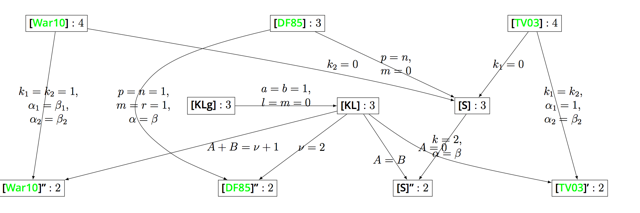
\includegraphics{intdep.png}} 
\end{question}

We list the formul{\ae}:
\begin{eqnarray}
  {}[\tmop{KLg}] : & \int_{(s, t) \in [- 1, 1]^2} | \varepsilon s a +
  \varepsilon' t b |^{2 \nu} u_l^{\lambda} (s) u_m^{\mu} (t) d s d t = & 
  \nonumber\\
  & \varepsilon^l (\varepsilon')^m (- \nu)_{\frac{l + m}{2}} (- 1)^{\frac{l +
  m}{2}} \pi^{3 / 2} \Gamma \left( \frac{1}{2} + \nu \right) \max^{2 \nu} \{ |
  a |, | b | \} \times &  \nonumber\\
  & \times \left\{ \begin{array}{ll}
    \frac{(b / a)^m _2 F_1 \left( \begin{array}{c}
      \frac{l + m}{2} - \nu, \frac{m - l}{2} - \nu - \lambda\\
      \mu + m + 1
    \end{array} ; \frac{b^2}{a^2} \right)}{\Gamma (\mu + m + 1) \Gamma \left(
    \nu + \frac{l - m}{2} + \lambda + 1 \right)}, & | b | \leqslant | a |,\\
    \frac{(a / b)^m _2 F_1 \left( \begin{array}{c}
      \frac{l + m}{2} - \nu, \frac{l - m}{2} - \nu - \mu\\
      \lambda + l + 1
    \end{array} ; \frac{a^2}{b^2} \right)}{\Gamma (\lambda + l + 1) \Gamma
    \left( \nu + \frac{m - l}{2} + \mu + 1 \right)}, & | a | \leqslant | b |,
  \end{array} \right. &  \nonumber\\
  {}[\tmop{KL}] : & \int_{(u, v) \in [- 1, 1]^2} | u - v |^{- \nu} (1 - u^2)^A
  (1 - v^2)^B d u d v = &  \nonumber\\
  & \frac{\Gamma \left( \frac{1 - \nu}{2} \right) \hspace{0.25em} \sqrt{\pi} 
  \hspace{0.25em} \Gamma (A + 1)  \hspace{0.25em} \Gamma (B + 1) 
  \hspace{0.25em} \Gamma (B + A - \nu + 2)}{\Gamma \left( \frac{2
  \hspace{0.25em} A - \nu + 3}{2} \right)  \hspace{0.25em} \Gamma \left(
  \frac{2 \hspace{0.25em} B - \nu + 3}{2} \right)  \hspace{0.25em} \Gamma
  \left( \frac{2 \hspace{0.25em} B + 2 \hspace{0.25em} A - \nu + 4}{2}
  \right)}, &  \nonumber\\
  \left[ \mathrm{S} \right] : & \int_{t \in [0, 1]^k} \Pi^{\alpha - 1, \beta -
  1} (t) \Delta^{2 \gamma} (t) d t = &  \nonumber\\
  & = \prod_{i = 0}^{k - 1} \frac{\Gamma (\alpha + i \gamma) \Gamma (\beta +
  i \gamma) \Gamma (1 + (i + 1) \gamma)}{\Gamma (\alpha + \beta + (i + k - 1)
  \gamma) \Gamma (\gamma + 1)}, &  \nonumber\\
  & \tmop{Re} (\alpha), \tmop{Re} (\beta) > 0, | \gamma | \ll 1 & 
  \nonumber\\
  \left[ \mathrm{S} \right]'' : & \int_{(t_1, t_2) \in [0, 1]^2} t_1^{\alpha -
  1} t_2^{\alpha - 1} (1 - t_1)^{\alpha - 1} (1 - t_2)^{\alpha - 1} | t_1 -
  t_2 |^{2 \gamma} d t_1 d t_2 = &  \nonumber\\
  & = \frac{\Gamma^2 (\alpha)}{\Gamma (2 \alpha + \gamma)} \cdot
  \frac{\Gamma^2 (\alpha + \gamma) \Gamma (1 + 2 \gamma)}{\Gamma (2 \alpha + 2
  \gamma) \Gamma (1 + \gamma)}, &  \nonumber\\
  \mathrm{{\cite[(1.4)]{warnaar2010sl3}}:} & \int_{(s, t) \in C_{\beta_1,
  \gamma}^{k_1, k_2} [0, 1]} \Pi^{\alpha_1 - 1, \beta_1 - 1} (t) \Pi^{\alpha_2
  - 1, \beta_2 - 1} (s) \Delta^{2 \gamma} (t) \Delta^{2 \gamma} (s) \Delta^{-
  \gamma} (s, t) d s d t = &  \nonumber\\
  & = \prod_{i = 0}^{k_1 - 1} \frac{\Gamma (\alpha_1 + i \gamma) \Gamma
  (\beta_1 + (i - k_2) \gamma) \Gamma ((i + 1) \gamma)}{\Gamma (\alpha_1 +
  \beta_1 + (i + k_1 - k_2 - 1) \gamma) \Gamma (\gamma)} \times &  \nonumber\\
  & \prod_{i = 0}^{k_2 - 1} \frac{\Gamma (\alpha_2 + i \gamma) \Gamma
  (\beta_2 + i \gamma) \Gamma ((i + 1) \gamma)}{\Gamma (\alpha_2 + \beta_2 +
  (i + k_2 - k_1 - 1) \gamma) \Gamma (\gamma)} \prod_{i = 0}^{k_1 - 1}
  \frac{\Gamma (\alpha_1 + \alpha_2 + (i - 1) \gamma)}{\Gamma (\alpha_1 +
  \alpha_2 + (i + k_2 - 1) \gamma)}, &  \nonumber\\
  & \beta_1 + \beta_2 = \gamma + 1 &  \nonumber\\
  & \tmop{Re} (\alpha_i), \tmop{Re} (\beta_i) > 0, | \gamma | \ll 1 ; \quad 1
  \leqslant \forall i \leqslant \min \{ k_i \}_i : \beta_1 + (i - k_2 - 1)
  \gamma \nin \mathbbm{Z} &  \nonumber\\
  \mathrm{{\cite{warnaar2010sl3}}}'' : & \int_{(s, t) \in C_{\alpha_1,
  \gamma}^{1, 1} [0, 1]} t^{\alpha_1 - 1} (1 - t)^{\alpha_1 - 1} s^{\alpha_2 -
  1} (1 - s)^{\alpha_2 - 1} | t - s |^{- \gamma} d s d t = &  \nonumber\\
  & = \frac{\Gamma (\alpha_1) \Gamma (\alpha_1 - \gamma)}{\Gamma (2 \alpha_1
  - \gamma)} \cdot \frac{\Gamma^2 (\alpha_2)}{\Gamma (2 \alpha_2 - \gamma)}
  \cdot \frac{\Gamma (\alpha_1 + \alpha_2 - \gamma)}{\Gamma (\alpha_1 +
  \alpha_1)} = &  \nonumber\\
  & \frac{\Gamma (\alpha_1) \Gamma (1 - \alpha_2)}{\Gamma (1 + \alpha_1 -
  \alpha_2)} \cdot \frac{\Gamma^2 (\alpha_2)}{\Gamma (1 + \alpha_2 -
  \alpha_1)} \cdot \frac{1}{\Gamma (\alpha_1 + \alpha_2)}, &  \nonumber\\
  & \alpha_1 + \alpha_2 = \gamma + 1, \quad C_{\alpha_1, \gamma}^{1, 1} [0,
  1] = \{ (t, s) \in [0, 1]^2 \mid t < s \} + \frac{\sin (\pi \alpha_1)}{\sin
  (\pi \alpha_2)} \{ (t, s) \in [0, 1]^2 \mid t > s \}, &  \nonumber\\
  \mathrm{{\cite[(3.3)]{tarasov2003selberg}}:} & \int_{(s, t) \in
  C_{\gamma}^{k_1, k_2}} \Pi^{\alpha_1 - 1, 0} (t) \Pi^{\alpha_2 - 1, \beta_2
  - 1} (s) \Delta^{2 \gamma} (t) \Delta^{2 \gamma} (s) \Delta^{- \gamma} (s,
  t) d s d t = &  \nonumber\\
  & \prod_{i = 0}^{k_1 - 1} \frac{\Gamma (\alpha_1 + i \gamma) \Gamma (1 + (i
  - k_2) \gamma) \Gamma ((i + 1) \gamma)}{\Gamma (\alpha_1 + 1 + (i + k_1 -
  k_2 - 1) \gamma) \Gamma (\gamma)} \times &  \nonumber\\
  & \prod_{i = 0}^{k_2 - 1} \frac{\Gamma (\alpha_2 + i \gamma) \Gamma
  (\beta_2 + i \gamma) \Gamma ((i + 1) \gamma)}{\Gamma (\alpha_2 + \beta_2 +
  (i + k_2 - k_1 - 1) \gamma) \Gamma (\gamma)} \times &  \nonumber\\
  & \prod_{i = 0}^{k_1 - 1} \frac{\Gamma (\alpha_1 + \alpha_2 + (i - 1)
  \gamma)}{\Gamma (\alpha_1 + \alpha_2 + \beta_2 + (i + k_2 - 2) \gamma)}
  \prod_{i = 0}^{k_1 - 1} \frac{\Gamma (\alpha_2 + \beta_2 + (i + k_2 - k_1 -
  1) \gamma)}{\Gamma (\alpha_2 + (i + k_2 - k_1) \gamma)} &  \nonumber\\
  & \tmop{Re} (\alpha_i), \tmop{Re} (\beta_2) > 0, | \tmop{Re} \gamma | \ll 1
  &  \nonumber\\
  \mathrm{{\cite{tarasov2003selberg}}}' : & \int_{(s, t) \in [0, 1]^2}
  s^{\alpha_2 - 1} (1 - s)^{\alpha_2 - 1} (t - s)_-^{- \gamma} d s d t =
  \frac{\Gamma (\alpha_2)}{(1 - \gamma)} \cdot \frac{\Gamma (1 + \alpha_2 -
  \gamma)}{\Gamma (1 + 2 \alpha_2 - \gamma)}, &  \nonumber\\
  \mathrm{{\cite[(A.35)]{dotsenko1985four}}:} & \frac{1}{n!m!} \int_{(t, \tau)
  \in [0, 1]^{n + m}} \Pi^{\alpha', \beta'} (t) \Pi^{\alpha, \beta} (\tau)
  \Delta^{2 \rho'} (t) \Delta^{2 \rho} (\tau) \Delta^{- 2} (t, \tau) d
  \tmop{td} \tau = &  \nonumber\\
  & \rho^{2 n m} \prod_{i, j = 1}^{n, m} \frac{1}{j \rho - i} \prod_{i = 1}^n
  \frac{\Gamma (i \rho')}{\Gamma (\rho')} \prod_{j = 1}^m \frac{\Gamma (j
  \rho)}{\Gamma (\rho)} \times &  \nonumber\\
  & \prod_{i, j = 0}^{n, m} \frac{1}{(\alpha + j \rho - i) (\beta + j \rho -
  i) (\alpha + \beta + \rho (m - 1 + j) - (n - 1 + i))} \times &  \nonumber\\
  & \prod_{i = 0}^{n - 1} \frac{\Gamma (1 + \alpha' + i \rho') \Gamma (1 +
  \beta' + i \rho')}{\Gamma (- 2 - 2 m + \alpha' + \beta' + (n - 1 + i)
  \rho')} \times &  \nonumber\\
  & \prod_{j = 0}^{m - 1} \frac{\Gamma (1 + \alpha + i \rho) \Gamma (1 +
  \beta + i \rho)}{\Gamma (2 - 2 n + \alpha + \beta + (m - 1 + i) \rho)}, & 
  \nonumber\\
  & \alpha' = - \rho' \alpha, \beta' = - \rho' \beta, \rho' \rho = 1, & 
  \nonumber\\
  & \tmop{Re} (\rho) < 0, \quad \tmop{Re} (\alpha), \tmop{Re} (\beta) > (n -
  1) + | \tmop{Re} (\rho) | (m - 1) &  \nonumber\\
  \mathrm{{\cite{dotsenko1985four}}}' : & \int_{(t, \tau) \in [0, 1]^2}
  t^{\alpha'} (1 - t)^{\alpha'} \tau^{\alpha} (1 - \tau)^{\alpha} | t - \tau
  |^{- 2} d \tmop{td} \tau = \frac{(\alpha / \alpha')^2}{(- \alpha / \alpha' -
  1)} \times &  \nonumber\\
  & \frac{1}{2 \alpha^4} \times \frac{\Gamma^2 (1 + \alpha')}{\Gamma (2
  \alpha')} \times \frac{\Gamma^2 (1 + \alpha)}{\Gamma (2 \alpha)} = & 
  \nonumber\\
  & \frac{- \pi / 2}{\alpha + \alpha'} \times \frac{\Gamma (1 +
  \alpha')}{2^{2 \alpha' - 1} \Gamma (\alpha' + 1 / 2)} \times \frac{\Gamma (1
  + \alpha)}{2^{2 \alpha - 1} \Gamma (\alpha + 1 / 2)}, &  \nonumber\\
  &  &  \nonumber\\
  & \Delta^{2 \gamma} (t) \assign \prod_{1 \leqslant i < j \leqslant k} | t_i
  - t_j |^{2 \gamma}, &  \nonumber\\
  & \Delta^{- \gamma}  (s, t) \assign \prod_{i, j = 1}^{k_1, k_2} | t_i - s_j
  |^{- \gamma}, &  \nonumber\\
  & \Pi^{x, y} (t) \assign \prod_{i = 1}^k t_i^x (1 - t_i)^y . &  \nonumber
\end{eqnarray}
We then prove some arrows of the diagram:
\begin{eqnarray}
  &
  \fbox{\concat{\math-up{[S]}}{<Rightarrow>}{\math-up{[S]}}{\rprime{''}}{:}}
  \tmop{obvious} &  \nonumber\\
  &
  \fbox{\concat{\math-up{[KL]}}{<Rightarrow>}{\math-up{[S]}}{\rprime{''}}{:}}
  \int_{(u, v) \in [- 1, 1]^2} | u - v |^{- \nu} (1 - u^2)^A (1 - v^2)^A d u d
  v = &  \nonumber\\
  & \frac{\Gamma \left( \frac{1 - \nu}{2} \right) \hspace{0.25em} \sqrt{\pi}
  \Gamma^2 (A + 1) \Gamma (2 A - \nu + 2)}{\Gamma^2 \left(
  \frac{\hspace{0.25em} 2 A - \nu + 3}{2} \right) \Gamma \left( \frac{4 A -
  \nu + 4}{2} \right)} \Leftrightarrow &  \nonumber\\
  & (u \rightarrow 2 t_1 - 1, v \rightarrow 2 t_2 - 1, \nu \rightarrow - 2
  \gamma, A \rightarrow \alpha - 1) &  \nonumber\\
  & 2^{2 \gamma - 2 + 4 \alpha} \int_{(t_1, t_2) \in [0, 1]^2} | t_1 - t_2
  |^{2 \gamma} t_1^{\alpha - 1} (1 - t_1)^{\alpha - 1} t_2^{\alpha - 1} (1 -
  t_2)^{\alpha - 1} d t_1 d t_2 = &  \nonumber\\
  & = \frac{\Gamma \left( \frac{1 + 2 \gamma}{2} \right) \hspace{0.25em}
  \sqrt{\pi} \Gamma^2 (\alpha) \Gamma (2 \alpha + 2 \gamma)}{\Gamma^2 \left(
  \frac{\hspace{0.25em} 2 \alpha + 1 + 2 \gamma}{2} \right) \Gamma \left(
  \frac{4 \alpha + 2 \gamma}{2} \right)} \Leftrightarrow &  \nonumber\\
  & 2^{2 \gamma - 2 + 4 \alpha} \int_{(t_1, t_2) \in [0, 1]^2} \ldots d t_1 d
  t_2 = \frac{2^{- 2 \gamma} \pi \Gamma (2 \gamma + 1) \Gamma^2 (\alpha)
  \Gamma (2 \alpha + 2 \gamma)}{\Gamma (\gamma + 1) \Gamma^2 \left(
  \frac{\hspace{0.25em} 2 \alpha + 1 + 2 \gamma}{2} \right) \Gamma \left(
  \frac{4 \alpha + 2 \gamma}{2} \right)} \Leftrightarrow &  \nonumber\\
  & 2^{2 \gamma - 1 + 2 \alpha} \int_{(t_1, t_2) \in [0, 1]^2} \ldots d t_1 d
  t_2 = \frac{\sqrt{\pi} \Gamma (2 \gamma + 1) \Gamma^2 (\alpha) \Gamma
  (\alpha + \gamma)}{\Gamma (\gamma + 1) \Gamma (2 \alpha + \gamma) \Gamma
  \left( \frac{2 \hspace{0.25em} \alpha + 1 + 2 \gamma}{2} \right)}
  \Leftrightarrow &  \nonumber\\
  & \int_{(t_1, t_2) \in [0, 1]^2} \ldots d t_1 d t_2 = \frac{\Gamma (2
  \gamma + 1) \Gamma^2 (\alpha) \Gamma^2 (\alpha + \gamma)}{\Gamma (\gamma +
  1) \Gamma (2 \alpha + \gamma) \Gamma (2 \alpha + 2 \gamma)} \Leftrightarrow
  \mathrm{[S]}'' ; &  \nonumber\\
  &
  \fbox{\concat{\math-up{\cite{warnaar2010sl3}}}{<Rightarrow>}{\math-up{\cite{warnaar2010sl3}}}{\rprime{''}}{:}}
  \tmop{obvious} &  \nonumber\\
  &
  \fbox{\concat{\math-up{[KL]}}{<Rightarrow>}{\math-up{\cite{warnaar2010sl3}}}{:}}
  \mathrm{ in fact, similarly to [KL] we can prove a bit more general:} & 
  \nonumber\\
  & \int_{(u, v) \in \{ [- 1, 1]^2 \mid \pm (u - v) > 0 \}} | u - v |^{- \nu}
  (1 - u^2)^A (1 - v^2)^B d u d v = &  \nonumber\\
  & \int_{(u, v) \in [- 1, 1]^2} (u - v)_{\pm}^{- \nu} (1 - u^2)^A (1 -
  v^2)^B d u d v = &  \nonumber\\
  & \frac{\Gamma \left( \frac{1 - \nu}{2} \right) \hspace{0.25em} \sqrt{\pi} 
  \hspace{0.25em} \Gamma (A + 1)  \hspace{0.25em} \Gamma (B + 1) 
  \hspace{0.25em} \Gamma (B + A - \nu + 2)}{2 \Gamma \left( \frac{2
  \hspace{0.25em} A - \nu + 3}{2} \right)  \hspace{0.25em} \Gamma \left(
  \frac{2 \hspace{0.25em} B - \nu + 3}{2} \right)  \hspace{0.25em} \Gamma
  \left( \frac{2 \hspace{0.25em} B + 2 \hspace{0.25em} A - \nu + 4}{2}
  \right)} \qquad (\tmop{KL} \pm), &  \nonumber\\
  & \mathrm{and similarly for [KLg]. Using that, we proceed as:} & 
  \nonumber\\
  & \tmop{LHS} \left( \mathrm{{\cite{warnaar2010sl3}}}'' \right) = \int_{(s,
  t) \in C_{\alpha_1, \gamma}^{1, 1} [0, 1]} t^{\alpha_1 - 1} (1 -
  t)^{\alpha_1 - 1} s^{\alpha_2 - 1} (1 - s)^{\alpha_2 - 1} | t - s |^{-
  \gamma} d s d t = &  \nonumber\\
  & \left( t \rightarrow \frac{1 + u}{2}, s \rightarrow \frac{1 + v}{2} ;
  \quad C_{\alpha_1, \gamma}^{1, 1} [0, 1] = \{ (t, s) \in [0, 1]^2 \mid t < s
  \} + \frac{\sin (\pi \alpha_1)}{\sin (\pi \alpha_2)} \{ (t, s) \in [0, 1]^2
  \mid t > s \} \right) &  \nonumber\\
  & \frac{1}{2^{2 \alpha_1 + 2 \alpha_2 - 2 - \gamma}}^{} \int_{(u, v) \in [-
  1, 1]^2} (1 - u^2)^{\alpha_1 - 1} (1 - v^2)^{\alpha_2 - 1} \left( (u -
  v)_+^{- \gamma} + \frac{\sin (\pi \alpha_1)}{\sin (\pi \alpha_2)} (u -
  v)_-^{- \gamma} \right) d u d v = &  \nonumber\\
  & ([\tmop{KL} \pm]) &  \nonumber\\
  & \frac{1}{2^{2 \alpha_1 + 2 \alpha_2 - 1 - \gamma}}^{} \cdot \frac{\Gamma
  \left( \frac{1 - \gamma}{2} \right) \hspace{0.25em} \sqrt{\pi} 
  \hspace{0.25em} \Gamma (\alpha_1)  \hspace{0.25em} \Gamma (\alpha_2) 
  \hspace{0.25em} \Gamma (\alpha_1 + \alpha_2 - \gamma)}{\Gamma \left( \frac{2
  \alpha_1 - \gamma + 1}{2} \right)  \hspace{0.25em} \Gamma \left( \frac{2
  \hspace{0.25em} \alpha_2 - \gamma + 1}{2} \right)  \hspace{0.25em} \Gamma
  \left( \frac{2 \hspace{0.25em} \alpha_1 + 2 \hspace{0.25em} \alpha_2 -
  \gamma}{2} \right)} \cdot \frac{2 \sin \left( \pi \frac{\alpha_1 +
  \alpha_2}{2} \right) \sin \left( \pi \frac{1 - \alpha_1 + \alpha_2}{2}
  \right)}{\sin (\pi \alpha_2)} = &  \nonumber\\
  & (\alpha_1 + \alpha_2 = \gamma + 1) &  \nonumber\\
  & \frac{1}{2^{\alpha_1 + \alpha_2}}^{} \cdot \frac{\Gamma \left( \frac{2 -
  \alpha_1 - \alpha_2}{2} \right) \hspace{0.25em} \sqrt{\pi}  \hspace{0.25em}
  \Gamma (\alpha_1)  \hspace{0.25em} \Gamma (\alpha_2)}{\Gamma \left(
  \frac{\alpha_1 - \alpha_2 + 2}{2} \right)  \hspace{0.25em} \Gamma \left(
  \frac{\alpha_1 - \alpha_2 + 2}{2} \right)  \hspace{0.25em} \Gamma \left(
  \frac{\alpha_1 + \alpha_2 + 1}{2} \right)} \cdot \frac{2 \sin \left( \pi
  \frac{\alpha_1 + \alpha_2}{2} \right) \sin \left( \pi \frac{1 - \alpha_1 +
  \alpha_2}{2} \right)}{\sin (\pi \alpha_2)} = &  \nonumber\\
  & \frac{1}{2^{\alpha_1 + \alpha_2}}^{} \cdot \frac{\hspace{0.25em} \pi^{3 /
  2}  \hspace{0.25em} \Gamma (\alpha_1)  \hspace{0.25em} \Gamma
  (\alpha_2)}{\Gamma \left( \frac{\alpha_1 - \alpha_2 + 2}{2} \right) 
  \hspace{0.25em} \Gamma \left( \frac{\alpha_1 - \alpha_2 + 2}{2} \right) 
  \hspace{0.25em} \Gamma \left( \frac{\alpha_1 + \alpha_2 + 1}{2} \right)}
  \cdot \frac{2 \sin \left( \pi \frac{1 - \alpha_1 + \alpha_2}{2}
  \right)}{\Gamma \left( \frac{\alpha_1 + \alpha_2}{2} \right) \sin (\pi
  \alpha_2)} = &  \nonumber\\
  & \frac{1}{2^{\alpha_1 + \alpha_2}}^{} \cdot \frac{\pi^{1 / 2} 
  \hspace{0.25em} \Gamma (\alpha_1)  \hspace{0.25em} \Gamma^2  (\alpha_2)
  \Gamma (1 - \alpha_2)}{\Gamma \left( \frac{\alpha_1 - \alpha_2 + 2}{2}
  \right)  \hspace{0.25em} \Gamma \left( \frac{\alpha_1 - \alpha_2 + 2}{2}
  \right)  \hspace{0.25em} \Gamma \left( \frac{\alpha_1 + \alpha_2 + 1}{2}
  \right)} \cdot \frac{2 \sin \left( \pi \frac{1 - \alpha_1 + \alpha_2}{2}
  \right)}{\Gamma \left( \frac{\alpha_1 + \alpha_2}{2} \right)} = & 
  \nonumber\\
  & \frac{\Gamma (\alpha_1)  \hspace{0.25em} \Gamma^2  (\alpha_2) \Gamma (1 -
  \alpha_2)}{\Gamma (\alpha_1 - \alpha_2 + 1)  \hspace{0.25em} \Gamma
  (\alpha_2 - \alpha_1 + 1)  \hspace{0.25em} \Gamma (\alpha_1 + \alpha_2)} =
  \tmop{RHS} \left( \mathrm{{\cite{warnaar2010sl3}}}'' \right) ; & 
  \nonumber\\
  &
  \fbox{\concat{\math-up{\cite{tarasov2003selberg}}}{<Rightarrow>}{\math-up{\cite{tarasov2003selberg}}}{\rprime{'}}}
  : \tmop{obvious} ; &  \nonumber\\
  &
  \fbox{\concat{\math-up{[KL]}}{<Rightarrow>}{\math-up{\cite{tarasov2003selberg}}}{\rprime{'}}}
  : \tmop{LHS} \left( \mathrm{{\cite{tarasov2003selberg}}}' \right) =
  \int_{(s, t) \in [0, 1]^2} s^{\alpha_2 - 1} (1 - s)^{\alpha_2 - 1} (t -
  s)_-^{- \gamma} d s d t = &  \nonumber\\
  & \left( t \rightarrow \frac{1 + u}{2}, s \rightarrow \frac{1 + v}{2}
  \right) &  \nonumber\\
  & \frac{1}{2^{2 \alpha_2 - \gamma}} \int_{(u, v) \in [- 1, 1]^2} (1 -
  v^2)^{\alpha_2 - 1} (u - v)_-^{- \gamma} d u d v = &  \nonumber\\
  & \left( \mathrm{[KL]} \right) &  \nonumber\\
  & \frac{\Gamma \left( \frac{1 - \gamma}{2} \right) \hspace{0.25em}
  \sqrt{\pi} \hspace{0.25em} \Gamma (\alpha_2)  \hspace{0.25em} \Gamma
  (\alpha_2 + 1 - \gamma)}{2^{2 \alpha_2 - \gamma + 1} \Gamma \left( \frac{3 -
  \gamma}{2} \right)  \hspace{0.25em} \Gamma \left( \frac{2 \hspace{0.25em}
  \alpha_2 - \gamma + 1}{2} \right)  \hspace{0.25em} \Gamma \left( \frac{2
  \hspace{0.25em} \alpha_2 + 2 - \gamma}{2} \right)} = \frac{\hspace{0.25em}
  \Gamma (\alpha_2)  \hspace{0.25em} \Gamma (\alpha_2 + 1 - \gamma)}{(1 -
  \gamma) \hspace{0.25em} \Gamma \left( 2 \hspace{0.25em} \alpha_2 - \gamma +
  1 \right)} = \tmop{RHS} \left( \mathrm{{\cite{tarasov2003selberg}}}' \right)
  ; &  \nonumber\\
  &
  \fbox{\concat{\math-up{\cite{dotsenko1985four}}}{<Rightarrow>}{\math-up{\cite{dotsenko1985four}}}{\rprime{'}}}
  : \tmop{obvious} &  \nonumber\\
  &
  \fbox{\concat{\math-up{[KL]}}{<Rightarrow>}{\math-up{\cite{dotsenko1985four}}}{\rprime{'}}}
  : \tmop{LHS} \left( \mathrm{{\cite{dotsenko1985four}}}' \right) = \int_{(t,
  \tau) \in [0, 1]^2} t^{\alpha'} (1 - t)^{\alpha'} \tau^{\alpha} (1 -
  \tau)^{\alpha} | t - \tau |^{- 2} d \tmop{td} \tau = &  \nonumber\\
  & \left( t \rightarrow \frac{1 + u}{2}, s \rightarrow \frac{1 + v}{2}
  \right) &  \nonumber\\
  & \frac{1}{2^{2 \alpha' + 2 \alpha}} \int_{(u, v) \in [- 1, 1]^2} (1 -
  u^2)^{\alpha'} (1 - v)^{\alpha} | u - v |^{- 2} d u d v = &  \nonumber\\
  & \left( \mathrm{[KL]} \right) &  \nonumber\\
  & \frac{1}{2^{2 \alpha' + 2 \alpha}} \frac{\Gamma (- 1 / 2) \sqrt{\pi}
  \Gamma (\alpha + 1) \Gamma (\alpha' + 1)}{\Gamma (\alpha + 1 / 2) \Gamma
  (\alpha' + 1 / 2) (\alpha' + \alpha)} = \frac{1}{2^{2 \alpha' + 2 \alpha}}
  \frac{- 2 \pi \Gamma (\alpha + 1) \Gamma (\alpha' + 1)}{\Gamma (\alpha + 1 /
  2) \Gamma (\alpha' + 1 / 2) (\alpha' + \alpha)} &  \nonumber\\
  & \frac{- \pi / 2}{\alpha + \alpha'} \times \frac{\Gamma (1 +
  \alpha')}{2^{2 \alpha' - 1} \Gamma (\alpha' + 1 / 2)} \times \frac{\Gamma (1
  + \alpha)}{2^{2 \alpha - 1} \Gamma (\alpha + 1 / 2)} = \tmop{RHS} \left(
  \mathrm{{\cite{dotsenko1985four}}}' \right) . &  \nonumber
\end{eqnarray}
\begin{question}
  What are the singular points of the ODE in Question \ref{q-ode}? What are
  exponents at these points?
\end{question}

Indeed, the ODE gets rewritten as:
\begin{eqnarray}
  & f'' + \frac{1 - 2 \lambda - (2 \lambda + 1) x}{1 - x^2} f' + \frac{(2 x +
  1) \left( \lambda^2 - \frac{1}{4} \right) + (l + 2 \lambda) (1 - x^2)}{(1 -
  x^2)^2} f = 0, &  \nonumber
\end{eqnarray}
thus one immediately sees that there are two candidates: $x = 1$ and $x = -
1$. We expand the coefficients around $x = 1$ first:
\begin{eqnarray}
  & \frac{1 - 2 \lambda - (2 \lambda + 1) x}{1 - x^2} = \frac{2 \lambda}{x -
  1} + \ldots, &  \nonumber\\
  & \frac{(2 x + 1) \left( \lambda^2 - \frac{1}{4} \right) + (l + 2 \lambda)
  (1 - x^2)}{(1 - x^2)^2} = \frac{3 \left( \lambda^2 - \frac{1}{4} \right) /
  4}{(x - 1)^2} + \ldots &  \nonumber
\end{eqnarray}
The indicial equation becomes:
\begin{eqnarray}
  & r (r - 1) + 2 \lambda r + \frac{3}{4} \left( \lambda^2 - \frac{1}{4}
  \right) = 0 \Leftrightarrow r^2 + 2 \left( \lambda + \frac{1}{2} \right) r +
  \frac{3 (\lambda^2 - 1 / 4)}{4} = 0, &  \nonumber
\end{eqnarray}
and the exponents are $r = - \left( \lambda + \frac{1}{2} \right) \pm
\frac{1}{2} \sqrt{\left( \lambda + \frac{7}{2} \right) \left( \lambda +
\frac{1}{2} \right)}$.

Then, around the $x = - 1$:
\begin{eqnarray}
  & \frac{1 - 2 \lambda - (2 \lambda + 1) x}{1 - x^2} = \frac{1}{x + 1} +
  \ldots, &  \nonumber\\
  & \frac{(2 x + 1) \left( \lambda^2 - \frac{1}{4} \right) + (l + 2 \lambda)
  (1 - x^2)}{(1 - x^2)^2} = \frac{- \left( \lambda^2 - \frac{1}{4} \right) /
  2}{(x + 1)^2} + \ldots, &  \nonumber
\end{eqnarray}
The indicial equuation becomes:
\begin{eqnarray}
  & r (r - 1) + r - \frac{1}{2} \left( \lambda^2 - \frac{1}{4} \right) = 0, &
  \nonumber
\end{eqnarray}
and the exponents are $r = \pm \frac{\sqrt{(\lambda - 1 / 2) (\lambda + 1 /
2)}}{\sqrt{2}}$.

Also, one sees that both singular points $x = \pm 1$ are regular.

\begin{corollary}
  \label{cor}{\tmdummy}
  
  \begin{eqnarray}
    & \int_{- 1}^1 \int_{- 1}^1 (s - t)_{\pm}^{2 \nu} (1 - s^2)^{\lambda -
    \frac{1}{2}} (1 - t^2)^{\mu - \frac{1}{2}} C_l^{\lambda} (s) C_m^{\mu} (t)
    d s d t = &  \nonumber\\
    & = \frac{\Gamma (2 \lambda + l) \Gamma (2 \mu + m) (- \nu)_{\frac{l +
    m}{2}} (- 1)^{\frac{l - m}{2}} \pi^{\frac{3}{2}} \Gamma \left( \frac{1}{2}
    + \nu \right) \Gamma (\mu + 1 + 2 \nu + \lambda)}{2^{2 \lambda + 2 \mu -
    1} l!m! \Gamma (\lambda) \Gamma (\mu) \Gamma \left( \nu + \frac{l - m}{2}
    + \lambda + 1 \right) \Gamma \left( \mu + 1 - \frac{l - m}{2} + \nu
    \right) \Gamma \left( \mu + 1 + \nu + \lambda + \frac{m + l}{2} \right)} =
    &  \nonumber\\
    & \frac{(2 \lambda)_l (2 \mu)_m \Gamma \left( \lambda + \frac{1}{2}
    \right) \Gamma \left( \mu + \frac{1}{2} \right) (- \nu)_{\frac{l + m}{2}}
    (- 1)^{\frac{l - m}{2}} \pi^{\frac{1}{2}} \Gamma \left( \frac{1}{2} + \nu
    \right) \Gamma (\mu + 1 + 2 \nu + \lambda)}{2 l!m! \Gamma \left( \nu +
    \frac{l - m}{2} + \lambda + 1 \right) \Gamma \left( \mu + 1 - \frac{l -
    m}{2} + \nu \right) \Gamma \left( \mu + 1 + \nu + \lambda + \frac{m +
    l}{2} \right)} . &  \nonumber
  \end{eqnarray}
\end{corollary}

\begin{question}
  \label{q14}Use the Corollary \ref{cor} to evaluate the integral
  \begin{eqnarray}
    & \int_{- \infty}^{\infty} \int_{- \infty}^{\infty} | x - y |^{2 \nu}
    e^{- x^2 - y^2} H_n (x) H_m (y) . &  \nonumber
  \end{eqnarray}
\end{question}

It equals to
\begin{eqnarray}
  &
  \fbox{\concat{\concat{\left{(}}{-<nu>}{\right{)}}}{\rsub{\frac{n+m}{2}}}{\concat{\left{(}}{-1}{\right{)}}}{\rsup{\frac{n-m}{2}}}{<pi>}{\rsup{\frac{1}{2}}}{<Gamma>}{\concat{\left{(}}{\frac{1}{2}}{+<nu>}{\right{)}}}{2}{\rsup{\concat{<nu>+}{\frac{m+n}{2}}}}{.}}
  &  \nonumber
\end{eqnarray}
Indeed,
\begin{eqnarray}
  & \int_{- 1}^1 \int_{- 1}^1 | s - t |^{2 \nu} (1 - s^2)^{\lambda -
  \frac{1}{2}} (1 - t^2)^{\mu - \frac{1}{2}} C_l^{\lambda} (s) C_m^{\mu} (t) d
  s d t = &  \nonumber\\
  & \frac{(2 \lambda)_l (2 \mu)_m \Gamma \left( \lambda + \frac{1}{2} \right)
  \Gamma \left( \mu + \frac{1}{2} \right) (- \nu)_{\frac{l + m}{2}} (-
  1)^{\frac{l - m}{2}} \pi^{\frac{1}{2}} \Gamma \left( \frac{1}{2} + \nu
  \right) \Gamma (\mu + 1 + 2 \nu + \lambda)}{l!m! \Gamma \left( \nu + \frac{l
  - m}{2} + \lambda + 1 \right) \Gamma \left( \mu + 1 - \frac{l - m}{2} + \nu
  \right) \Gamma \left( \mu + 1 + \nu + \lambda + \frac{m + l}{2} \right)}
  \Rightarrow &  \nonumber\\
  & \left( s \rightarrow \frac{x}{\sqrt{\lambda}}, t \rightarrow
  \frac{y}{\sqrt{\mu}}, \mu \rightarrow \lambda \right) &  \nonumber\\
  & \int_{- \sqrt{\lambda}}^{\sqrt{\lambda}} \int_{-
  \sqrt{\lambda}}^{\sqrt{\lambda}} | x - y |^{2 \nu} \left( 1 -
  \frac{x^2}{\lambda} \right)^{\lambda - \frac{1}{2}} \left( 1 -
  \frac{y^2}{\lambda} \right)^{\lambda - \frac{1}{2}} C_l^{\lambda} \left(
  \frac{x}{\sqrt{\lambda}} \right) C_m^{\lambda} \left(
  \frac{y}{\sqrt{\lambda}} \right) d x d y = &  \nonumber\\
  & \frac{\lambda^{1 + \nu} (2 \lambda)_l (2 \lambda)_m \Gamma \left( \lambda
  + \frac{1}{2} \right)^2 (- \nu)_{\frac{l + m}{2}} (- 1)^{\frac{l - m}{2}}
  \pi^{\frac{1}{2}} \Gamma \left( \frac{1}{2} + \nu \right) \Gamma (1 + 2 \nu
  + 2 \lambda)}{l!m! \Gamma \left( \nu + \frac{l - m}{2} + \lambda + 1 \right)
  \Gamma \left( \lambda + 1 - \frac{l - m}{2} + \nu \right) \Gamma \left( 1 +
  \nu + 2 \lambda + \frac{m + l}{2} \right)} \Rightarrow &  \nonumber\\
  & \left( l \rightarrow n \quad ; \lambda \rightarrow \infty ; \quad
  \lambda^{- \frac{n}{2}} C_n^{\lambda} \left( \frac{x}{\sqrt{\lambda}}
  \right) \rightarrow \frac{H_n (x)}{n!}, \; \left( 1 - \frac{x^2}{\lambda}
  \right)^{\lambda - \frac{1}{2}} \rightarrow e^{- x^2} \right) &  \nonumber\\
  &
  \fbox{\concat{\big{int}}{\rsub{-<infty>}}{\rsup{<infty>}}{\big{int}}{\rsub{-<infty>}}{\rsup{<infty>}}{\concat{\left{|}}{x-y}{\right{|}}}{\rsup{2<nu>}}{e}{\rsup{\concat{-x}{\rsup{2}}{-y}{\rsup{2}}}}{H}{\rsub{n}}{\concat{\left{(}}{x}{\right{)}}}{H}{\rsub{m}}{\concat{\left{(}}{y}{\right{)}}}{d
  x d y}} = (- \nu)_{\frac{n + m}{2}} (- 1)^{\frac{n - m}{2}}
  \pi^{\frac{1}{2}} \Gamma \left( \frac{1}{2} + \nu \right) &  \nonumber\\
  & \lim_{\lambda \rightarrow \infty} \frac{\lambda^{1 + \nu - \frac{m +
  n}{2}} (2 \lambda)_n (2 \lambda)_m \Gamma \left( \lambda + \frac{1}{2}
  \right)^2 \Gamma (1 + 2 \nu + 2 \lambda)}{\Gamma \left( \nu + \frac{n -
  m}{2} + \lambda + 1 \right) \Gamma \left( \lambda + 1 - \frac{n - m}{2} +
  \nu \right) \Gamma \left( 1 + \nu + 2 \lambda + \frac{m + n}{2} \right)} = &
  \nonumber\\
  & \left( \Gamma (z + a) / \Gamma (z + b) \sim z^{a - b}, \quad (2
  \lambda)_n \sim 2^n \lambda^n \right) &  \nonumber\\
  & (- \nu)_{\frac{n + m}{2}} (- 1)^{\frac{n - m}{2}} \pi^{\frac{1}{2}}
  \Gamma \left( \frac{1}{2} + \nu \right) 2^{n + m} \lim_{\lambda \rightarrow
  \infty} \left( \lambda^{1 + \nu + \frac{m + n}{2}} \lambda^{\frac{1}{2} -
  \left( \nu + \frac{n - m}{2} + 1 \right)} \lambda^{\frac{1}{2} - 1 - \frac{n
  - m}{2} + \nu} (2 \lambda)^{1 + 2 \nu - 1 - \nu - \frac{m + n}{2}} \right) =
  &  \nonumber\\
  & (- \nu)_{\frac{n + m}{2}} (- 1)^{\frac{n - m}{2}} \pi^{\frac{1}{2}}
  \Gamma \left( \frac{1}{2} + \nu \right) 2^{n + m} 2^{\nu - \frac{m + n}{2}}
  \lim_{\lambda \rightarrow \infty} \left( \lambda^{1 + \nu + \frac{m + n}{2}}
  \lambda^{- 1} \lambda^{\nu - \frac{m + n}{2}} \right) = &  \nonumber\\
  &
  \fbox{\concat{\concat{\left{(}}{-<nu>}{\right{)}}}{\rsub{\frac{n+m}{2}}}{\concat{\left{(}}{-1}{\right{)}}}{\rsup{\frac{n-m}{2}}}{<pi>}{\rsup{\frac{1}{2}}}{<Gamma>}{\concat{\left{(}}{\frac{1}{2}}{+<nu>}{\right{)}}}{2}{\rsup{\concat{<nu>+}{\frac{m+n}{2}}}}}
  . &  \nonumber
\end{eqnarray}
\begin{question}
  Check the correctness of the computations in Question \ref{q14}.
\end{question}

To this end, we provide the another proof of the equality of Question
\ref{q14}:
\begin{eqnarray}
  & \int_{- \infty}^{\infty} \int_{- \infty}^{\infty} | x - y |^{2 \nu} e^{-
  x^2 - y^2} H_n (x) H_m (y) d x d y = &  \nonumber\\
  & \left( H_n (x) = (- 1)^n e^{x^2} \frac{d^n}{d x^n} e^{- x^2} \right) & 
  \nonumber\\
  & \int_{- \infty}^{\infty} \int_{- \infty}^{\infty} | x - y |^{2 \nu} e^{-
  x^2 - y^2} \frac{\partial}{\partial x^n} e^{- x^2} \frac{\partial}{\partial
  x^m} e^{- x^2} d x d y = &  \nonumber\\
  & (\tmop{integration} \tmop{by} \tmop{parts}) &  \nonumber\\
  & (- 1)^m (- 2 \nu)_{n + m} \int_{- \infty}^{\infty} \int_{-
  \infty}^{\infty} | x - y |^{2 \nu - n - m} e^{- x^2 - y^2} d x d y = & 
  \nonumber\\
  & \left( \mathrm{Mehta's integral:} \int_{t \in \mathbbm{R}^n} \Delta^{2
  \gamma} (t) e^{- | t |^2 / 2} d t = (2 \pi)^{n / 2} \prod_{j = 1}^n
  \frac{\Gamma (1 + j \gamma)}{\Gamma (1 + \gamma)} \right) &  \nonumber\\
  & (- 1)^m (- 2 \nu)_{n + m} 2^{\frac{n + m}{2} - \nu} \pi \frac{\Gamma (1 +
  2 \nu - n - m)}{\Gamma \left( 1 + \nu - \frac{n + m}{2} \right)} = \frac{(-
  1)^m 2^{\frac{n + m}{2} - \nu} \pi \Gamma (n + m - 2 \nu) \Gamma (1 + 2 \nu
  - n - m)}{\Gamma (- 2 \nu) \Gamma \left( 1 + \nu - \frac{n + m}{2} \right)}
  = &  \nonumber\\
  & \frac{(- 1)^m 2^{\frac{n + m}{2} - \nu} \pi \Gamma (1 + 2 \nu)}{\Gamma
  \left( 1 + \nu - \frac{n + m}{2} \right)} = \frac{(- 1)^m \sqrt{\pi}
  2^{\frac{n + m}{2} + \nu} \Gamma \left( \nu + \frac{1}{2} \right) \Gamma
  (\nu + 1)}{\Gamma \left( 1 + \nu - \frac{n + m}{2} \right)} = &  \nonumber\\
  & \frac{(- 1)^{\frac{n - m}{2}} \sqrt{\pi} 2^{\nu + \frac{n + m}{2}} \Gamma
  \left( \frac{1}{2} + \nu \right) \Gamma \left( \frac{n + m}{2} - \nu
  \right)}{\Gamma (- \nu)} = (- \nu)_{\frac{n + m}{2}} (- 1)^{\frac{n - m}{2}}
  \pi^{\frac{1}{2}} 2^{\nu + \frac{n + m}{2}} \Gamma \left( \frac{1}{2} + \nu
  \right) . &  \nonumber\\
  &  &  \nonumber
\end{eqnarray}
\begin{question}
  Is the equality of the Question \ref{q14} can be found in some other
  published work?
\end{question}

I have not found explicit reference yet. ``Mathematica'' software seems to not
know this equality. Nevertheless, I have found references
\href{http://functions.wolfram.com/Polynomials/HermiteH/21/02/01/0008/}{on the
web} for the equality:
\begin{eqnarray}
  &  &  \nonumber
\end{eqnarray}
\begin{thebibliography}{War10}
  \bibitem[DF85]{dotsenko1985four}Vl~S Dotsenko and Vladimir~A Fateev.
  {\newblock}Four-point correlation functions and the operator algebra in 2d
  conformal invariant theories with central charge $c \leq 1$.
  {\newblock}\tmtextit{Nuclear Physics B}, 251:691--734, 1985.
  
  \bibitem[TV03]{tarasov2003selberg}V~Tarasov and Alexander Varchenko.
  {\newblock}Selberg-type integrals associated with sl 3.
  {\newblock}\tmtextit{Letters in Mathematical Physics}, 65(3):173--185, 2003.
  
  \bibitem[War10]{warnaar2010sl3}S~Ole Warnaar. {\newblock}The sl3 selberg
  integral. {\newblock}\tmtextit{Advances in Mathematics}, 224(2):499--524,
  2010.
\end{thebibliography}

\end{document}
